\section{Bước 4: Thiết kế bản đồ mạng trên Cisco Packet Tracer}
\label{sec:step4}

Phần mềm mô phỏng là \textbf{Cisco Packet Tracer 9.0.1}. Tên thiết bị theo sơ đồ chuẩn trong hình~\ref{fig:topology}.

\subsection{Tổng quan topology}
\label{sec:step4-topology}

Sơ đồ gồm 29 thiết bị mạng (router, switch, firewall, WLC) cùng các thiết bị đầu cuối, chia thành 4 vùng:

\begin{small}
\setlength{\tabcolsep}{4pt}
\begin{longtable}{|p{3.6cm}|p{10.2cm}|}
\caption{Các vùng trong topology mô phỏng} \label{tab:topo_zones} \\
\hline
\textbf{Vùng} & \textbf{Thiết bị} \\ \hline
\endhead
Main Site -- lõi và truy cập & \texttt{MAIN-CORE-SW1/2}, \texttt{Server-SW}, \texttt{Mgmt-SW}, \texttt{Cam-SW}, \texttt{SW-MAIN-A}, \texttt{SW-MAIN-B}, \texttt{MAIN-R}, \texttt{MAIN-WLC} \\ \hline
Main Site -- biên, DMZ, WAN & \texttt{MAIN-FW-01}, \texttt{MAIN-FW-02}, \texttt{MAIN-VPN}, \texttt{DMZ-SW}, \texttt{MAIN-WAN1-SW}, \texttt{MAIN-WAN2-SW}, \texttt{MAIN-WAN-R1/R2}, \texttt{ISP1-R}, \texttt{ISP1-SW} \\ \hline
Backbone WAN & \texttt{Carrier-R} (leased line/MPLS giả lập), \texttt{ISP2-R} (broadband giả lập) \\ \hline
Chi nhánh & \texttt{DBP-R1/R2}, \texttt{DBP-SW1/SW2}; \texttt{BHTQ-R1/R2}, \texttt{BHTQ-SW1/SW2} \\ \hline
\end{longtable}
\end{small}

\noindent Hai firewall nối tiếp theo mô hình screened subnet: \texttt{Internet -- ISP1-R -- MAIN-FW-02 -- DMZ-SW -- MAIN-FW-01 -- Core/WAN}. \texttt{MAIN-VPN} đặt ở vùng Internet Edge, nối \texttt{ISP1-SW}, \texttt{DMZ-SW} và \texttt{MAIN-FW-01}.

\begin{sidewaysfigure}
    \centering
    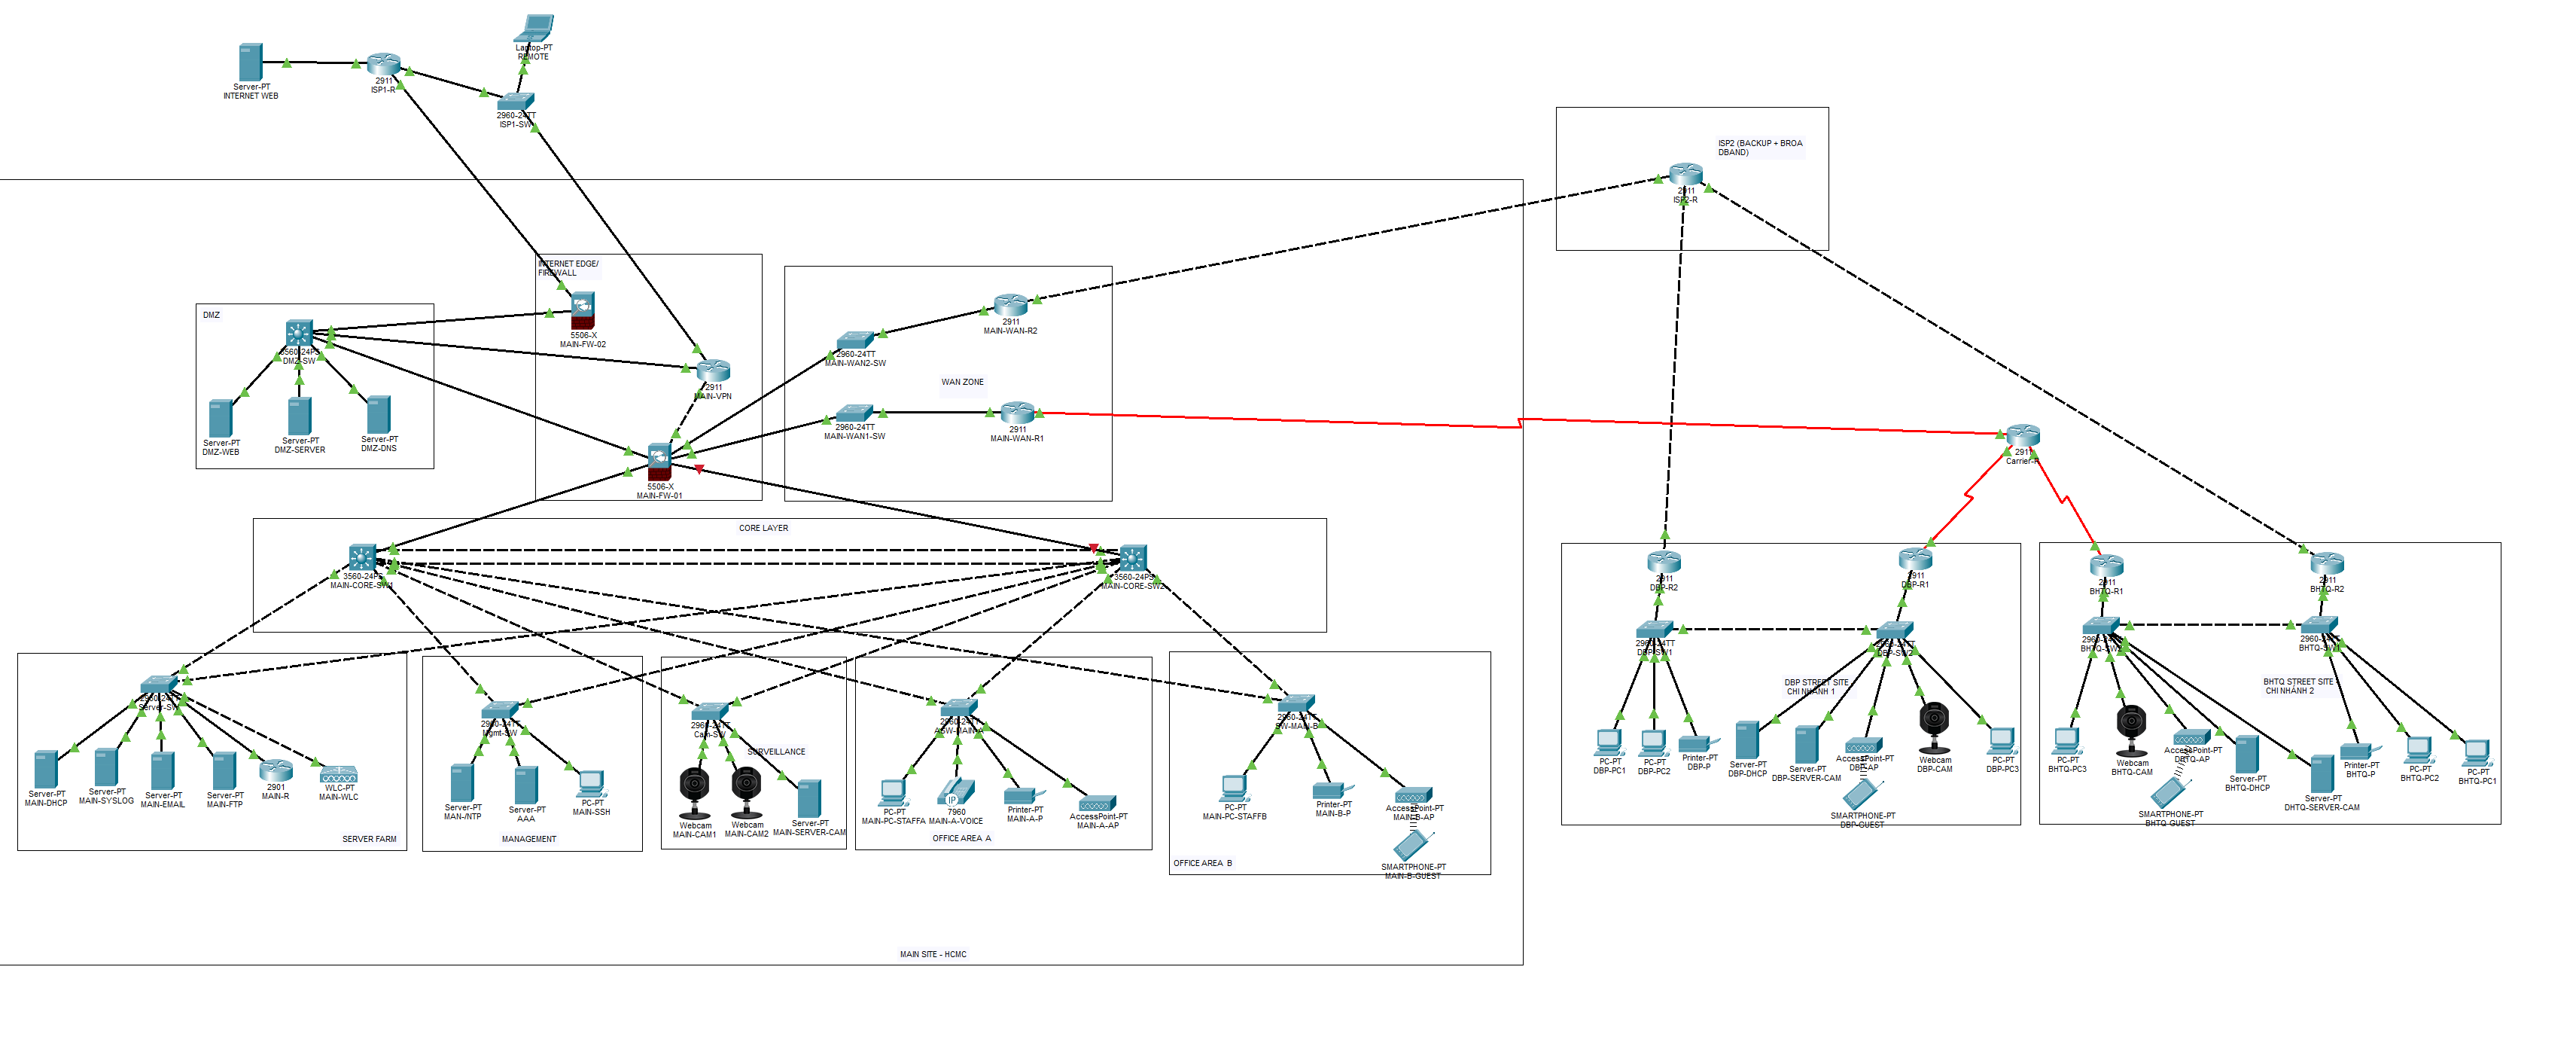
\includegraphics[width=\linewidth]{graphics/topology.png}
    \caption{Sơ đồ topology mô phỏng trên Cisco Packet Tracer (sơ đồ chuẩn)}
    \label{fig:topology}
\end{sidewaysfigure}

\subsection{Các tính năng đã mô phỏng}
\begin{small}
\setlength{\tabcolsep}{4pt}
\begin{longtable}{|p{2.2cm}|p{7.8cm}|p{3.8cm}|}
\caption{Các tính năng đã mô phỏng} \label{tab:sim_features} \\
\hline
\textbf{Nhóm} & \textbf{Tính năng} & \textbf{Thiết bị chính} \\ \hline
\endhead
Lớp 2 & VLAN, trunk 802.1Q, Rapid-PVST, LACP Port-channel 1 giữa hai Core & Core, Access \\ \hline
Dự phòng cổng & HSRP (Core: prio 200/150; chi nhánh: 110/105, \texttt{standby track Serial0/3/0}) & \texttt{MAIN-CORE-SW1/2}, \texttt{DBP/BHTQ-R1/R2} \\ \hline
Định tuyến & OSPF Area 0 (leased line, cost 10); static và default; floating static AD 150 (chi nhánh) và AD 10 (\texttt{MAIN-FW-01}) & \texttt{MAIN-WAN-R1}, \texttt{Carrier-R}, router chi nhánh \\ \hline
Firewall & Zone và security level: inside 100, inside-backup 100, wan 70, backup-wan 60, dmz 50, outside 0 & \texttt{MAIN-FW-01}, \texttt{MAIN-FW-02} \\ \hline
NAT & Static NAT \texttt{10.10.50.10} $\leftrightarrow$ \texttt{203.162.10.3} (TCP/80); PAT cho \texttt{10.0.0.0/8} ra Internet & \texttt{MAIN-FW-02} \\ \hline
ACL & \texttt{ACL-GUEST-ISOLATE} cho VLAN 60 (cần áp dụng lại, xem Bước~5 và 6) & Core \\ \hline
DHCP & Main Site: DHCP relay từ SVI tới \texttt{MAIN-DHCP}; mỗi chi nhánh có máy chủ DHCP cục bộ (\texttt{DBP-DHCP}, \texttt{BHTQ-DHCP}) & Core, \texttt{DBP-DHCP}, \texttt{BHTQ-DHCP} \\ \hline
VPN & IPsec site-to-site giữa router WAN; remote-access VPN (client nhận \texttt{10.10.200.10}) & \texttt{MAIN-WAN-R2}, \texttt{MAIN-VPN}, \texttt{REMOTE} \\ \hline
Không dây & Access Point và WLC, SSID staff và guest & Access, Server Farm (\texttt{MAIN-WLC}) \\ \hline
Giám sát & Syslog (\texttt{MAIN-SYSLOG}, \texttt{10.10.40.11}) và NTP (\texttt{MAIN-NTP}, \texttt{10.10.90.20}) & Server Farm, Management \\ \hline
\end{longtable}
\end{small}

\subsection{Cấu hình quan trọng (trích)}

\subsubsection{HSRP và tracking ở chi nhánh}
\begin{lstlisting}[language=csh,caption={Subinterface VLAN 10 trên router chính chi nhánh}]
interface GigabitEthernet0/0.10
 encapsulation dot1Q 10
 ip address 10.20.10.2 255.255.255.0
 standby version 2
 standby 10 ip 10.20.10.1
 standby 10 priority 110
 standby 10 preempt
 standby 10 track Serial0/3/0 60
\end{lstlisting}
Router R2 dùng \texttt{standby 10 priority 105} và không cần \texttt{track}.

\subsubsection{OSPF trên liên kết leased line}
\begin{lstlisting}[language=csh,caption={OSPF trên DBP-R1}]
router ospf 1
 router-id 3.3.3.1
 network 10.255.0.8 0.0.0.3 area 0
 network 10.20.0.0 0.0.255.255 area 0
!
interface Serial0/3/0
 ip ospf cost 10
\end{lstlisting}

\subsubsection{Đường dự phòng (floating static)}
\begin{lstlisting}[language=csh,caption={Floating static tại chi nhánh và route trên MAIN-FW-01}]
! Tren DBP-R2
ip route 0.0.0.0 0.0.0.0 10.255.0.17 150
! Tren MAIN-FW-01
route backup-wan 10.20.0.0 255.255.0.0 10.10.252.4 10
route wan        10.20.0.0 255.255.0.0 10.10.251.3 1
\end{lstlisting}

\subsubsection{NAT trên MAIN-FW-02}
\begin{lstlisting}[language=csh,caption={Static NAT và PAT trên MAIN-FW-02}]
object network WEB-SERVER
 host 10.10.50.10
 nat (dmz,outside) static 203.162.10.3
object network INTERNAL-NET
 subnet 10.0.0.0 255.0.0.0
 nat (dmz,outside) dynamic interface
route outside 0.0.0.0 0.0.0.0 203.162.10.1
route dmz 10.0.0.0 255.0.0.0 10.10.50.1
\end{lstlisting}
\noindent Cấu hình đầy đủ nằm trong \texttt{running-config} của các thiết bị; hostname trong cấu hình cần được đồng bộ với tên thiết bị trên sơ đồ (xem Bước~6).

\subsection{Hạn chế của Packet Tracer ảnh hưởng thiết kế}
\begin{small}
\setlength{\tabcolsep}{4pt}
\begin{longtable}{|p{3.4cm}|p{2.8cm}|p{7.4cm}|}
\caption{Hạn chế của Packet Tracer và cách xử lý} \label{tab:pt_limits} \\
\hline
\textbf{Yêu cầu thiết kế đích} & \textbf{Tình trạng trong PT} & \textbf{Cách xử lý} \\ \hline
\endhead
Failover firewall (HA) & Không có & Hai ASA độc lập, ghi vào mục vấn đề còn lại \\ \hline
IPS/IDS & Không có & Ghi trong thiết kế đích, không mô phỏng \\ \hline
Load balancer & Không có & Nhiều Server-PT hoặc DNS round-robin; ghi thuyết minh \\ \hline
SD-WAN / MPLS thật & Không có & Mô phỏng bằng leased line + floating static \\ \hline
Thiết bị y tế & Không có mô hình & VLAN 30 chỉ quy hoạch và cấu hình gateway, không có thiết bị đầu cuối \\ \hline
Subinterface trên ASA & Không dùng & Mỗi vùng một cổng vật lý (ASA 5506-X có 8 cổng) \\ \hline
\end{longtable}
\end{small}

\subsection{Tên thiết bị đầu cuối}
Báo cáo bản trước dùng nhiều tên không thống nhất cho máy đầu cuối (\texttt{PC\_DATA}, \texttt{PC-BHTQ1}, \texttt{PC-BHTQ3}, \dots). Từ bản này, tên máy đầu cuối theo sơ đồ chuẩn: \texttt{MAIN-PC-STAFFA}, \texttt{MAIN-PC-STAFFB}, \texttt{MAIN-B-GUEST}, \texttt{REMOTE}, \texttt{DBP-PC1/2/3}, \texttt{BHTQ-PC1/2/3}. Một số ảnh kiểm thử cũ vẫn hiển thị tên hoặc hostname phiên bản trước (\texttt{Core-SW1}, \texttt{WAN-R2}, \texttt{VPN-GW}); danh sách ảnh cần chụp lại nằm trong tài liệu kèm theo.

\subsection{Các lỗi mô phỏng đã xử lý}
\begin{small}
\setlength{\tabcolsep}{4pt}
\begin{longtable}{|p{3.4cm}|p{4.4cm}|p{6.0cm}|}
\caption{Các lỗi mô phỏng đã gặp và cách sửa} \label{tab:sim_errors} \\
\hline
\textbf{Lỗi} & \textbf{Nguyên nhân} & \textbf{Cách sửa} \\ \hline
\endhead
\texttt{BHTQ-R2} không thấy \texttt{10.20.40.0/24} & Default static AD 1 đè OSPF gây bất đối xứng & Đổi thành floating AD 150, bỏ \texttt{default-information originate}, \texttt{passive-interface} trên cổng broadband \\ \hline
OSPF kẹt INIT/DROTHER qua VLAN 99 & \texttt{dot1Q native} kết hợp HSRP/OSPF trên subinterface & Bỏ \texttt{native}, dùng \texttt{dot1Q 99}, native VLAN của switch về 1 \\ \hline
HSRP nhóm 90 báo Speak & Thiếu subinterface Gi0/0.90 và allowed VLAN trên trunk & Khai báo đồng bộ trên cả R1/R2, mở trunk VLAN 1, 10, 30, 40, 70, 90, 99 \\ \hline
Không tới Server BHTQ \texttt{10.30.40.10} & Server thiếu default gateway & Đặt gateway \texttt{10.30.40.1}, gán access VLAN 40 \\ \hline
\end{longtable}
\end{small}
